% Options for packages loaded elsewhere
\PassOptionsToPackage{unicode}{hyperref}
\PassOptionsToPackage{hyphens}{url}
%
\documentclass[
]{book}
\usepackage{lmodern}
\usepackage{amssymb,amsmath}
\usepackage{ifxetex,ifluatex}
\ifnum 0\ifxetex 1\fi\ifluatex 1\fi=0 % if pdftex
  \usepackage[T1]{fontenc}
  \usepackage[utf8]{inputenc}
  \usepackage{textcomp} % provide euro and other symbols
\else % if luatex or xetex
  \usepackage{unicode-math}
  \defaultfontfeatures{Scale=MatchLowercase}
  \defaultfontfeatures[\rmfamily]{Ligatures=TeX,Scale=1}
\fi
% Use upquote if available, for straight quotes in verbatim environments
\IfFileExists{upquote.sty}{\usepackage{upquote}}{}
\IfFileExists{microtype.sty}{% use microtype if available
  \usepackage[]{microtype}
  \UseMicrotypeSet[protrusion]{basicmath} % disable protrusion for tt fonts
}{}
\makeatletter
\@ifundefined{KOMAClassName}{% if non-KOMA class
  \IfFileExists{parskip.sty}{%
    \usepackage{parskip}
  }{% else
    \setlength{\parindent}{0pt}
    \setlength{\parskip}{6pt plus 2pt minus 1pt}}
}{% if KOMA class
  \KOMAoptions{parskip=half}}
\makeatother
\usepackage{xcolor}
\IfFileExists{xurl.sty}{\usepackage{xurl}}{} % add URL line breaks if available
\IfFileExists{bookmark.sty}{\usepackage{bookmark}}{\usepackage{hyperref}}
\hypersetup{
  pdftitle={Introduction to Computational Biomedicine},
  pdfauthor={ERASMUS+ OERCompBioMed network},
  hidelinks,
  pdfcreator={LaTeX via pandoc}}
\urlstyle{same} % disable monospaced font for URLs
\usepackage{color}
\usepackage{fancyvrb}
\newcommand{\VerbBar}{|}
\newcommand{\VERB}{\Verb[commandchars=\\\{\}]}
\DefineVerbatimEnvironment{Highlighting}{Verbatim}{commandchars=\\\{\}}
% Add ',fontsize=\small' for more characters per line
\usepackage{framed}
\definecolor{shadecolor}{RGB}{248,248,248}
\newenvironment{Shaded}{\begin{snugshade}}{\end{snugshade}}
\newcommand{\AlertTok}[1]{\textcolor[rgb]{0.94,0.16,0.16}{#1}}
\newcommand{\AnnotationTok}[1]{\textcolor[rgb]{0.56,0.35,0.01}{\textbf{\textit{#1}}}}
\newcommand{\AttributeTok}[1]{\textcolor[rgb]{0.77,0.63,0.00}{#1}}
\newcommand{\BaseNTok}[1]{\textcolor[rgb]{0.00,0.00,0.81}{#1}}
\newcommand{\BuiltInTok}[1]{#1}
\newcommand{\CharTok}[1]{\textcolor[rgb]{0.31,0.60,0.02}{#1}}
\newcommand{\CommentTok}[1]{\textcolor[rgb]{0.56,0.35,0.01}{\textit{#1}}}
\newcommand{\CommentVarTok}[1]{\textcolor[rgb]{0.56,0.35,0.01}{\textbf{\textit{#1}}}}
\newcommand{\ConstantTok}[1]{\textcolor[rgb]{0.00,0.00,0.00}{#1}}
\newcommand{\ControlFlowTok}[1]{\textcolor[rgb]{0.13,0.29,0.53}{\textbf{#1}}}
\newcommand{\DataTypeTok}[1]{\textcolor[rgb]{0.13,0.29,0.53}{#1}}
\newcommand{\DecValTok}[1]{\textcolor[rgb]{0.00,0.00,0.81}{#1}}
\newcommand{\DocumentationTok}[1]{\textcolor[rgb]{0.56,0.35,0.01}{\textbf{\textit{#1}}}}
\newcommand{\ErrorTok}[1]{\textcolor[rgb]{0.64,0.00,0.00}{\textbf{#1}}}
\newcommand{\ExtensionTok}[1]{#1}
\newcommand{\FloatTok}[1]{\textcolor[rgb]{0.00,0.00,0.81}{#1}}
\newcommand{\FunctionTok}[1]{\textcolor[rgb]{0.00,0.00,0.00}{#1}}
\newcommand{\ImportTok}[1]{#1}
\newcommand{\InformationTok}[1]{\textcolor[rgb]{0.56,0.35,0.01}{\textbf{\textit{#1}}}}
\newcommand{\KeywordTok}[1]{\textcolor[rgb]{0.13,0.29,0.53}{\textbf{#1}}}
\newcommand{\NormalTok}[1]{#1}
\newcommand{\OperatorTok}[1]{\textcolor[rgb]{0.81,0.36,0.00}{\textbf{#1}}}
\newcommand{\OtherTok}[1]{\textcolor[rgb]{0.56,0.35,0.01}{#1}}
\newcommand{\PreprocessorTok}[1]{\textcolor[rgb]{0.56,0.35,0.01}{\textit{#1}}}
\newcommand{\RegionMarkerTok}[1]{#1}
\newcommand{\SpecialCharTok}[1]{\textcolor[rgb]{0.00,0.00,0.00}{#1}}
\newcommand{\SpecialStringTok}[1]{\textcolor[rgb]{0.31,0.60,0.02}{#1}}
\newcommand{\StringTok}[1]{\textcolor[rgb]{0.31,0.60,0.02}{#1}}
\newcommand{\VariableTok}[1]{\textcolor[rgb]{0.00,0.00,0.00}{#1}}
\newcommand{\VerbatimStringTok}[1]{\textcolor[rgb]{0.31,0.60,0.02}{#1}}
\newcommand{\WarningTok}[1]{\textcolor[rgb]{0.56,0.35,0.01}{\textbf{\textit{#1}}}}
\usepackage{longtable,booktabs}
% Correct order of tables after \paragraph or \subparagraph
\usepackage{etoolbox}
\makeatletter
\patchcmd\longtable{\par}{\if@noskipsec\mbox{}\fi\par}{}{}
\makeatother
% Allow footnotes in longtable head/foot
\IfFileExists{footnotehyper.sty}{\usepackage{footnotehyper}}{\usepackage{footnote}}
\makesavenoteenv{longtable}
\usepackage{graphicx,grffile}
\makeatletter
\def\maxwidth{\ifdim\Gin@nat@width>\linewidth\linewidth\else\Gin@nat@width\fi}
\def\maxheight{\ifdim\Gin@nat@height>\textheight\textheight\else\Gin@nat@height\fi}
\makeatother
% Scale images if necessary, so that they will not overflow the page
% margins by default, and it is still possible to overwrite the defaults
% using explicit options in \includegraphics[width, height, ...]{}
\setkeys{Gin}{width=\maxwidth,height=\maxheight,keepaspectratio}
% Set default figure placement to htbp
\makeatletter
\def\fps@figure{htbp}
\makeatother
\setlength{\emergencystretch}{3em} % prevent overfull lines
\providecommand{\tightlist}{%
  \setlength{\itemsep}{0pt}\setlength{\parskip}{0pt}}
\setcounter{secnumdepth}{5}
\usepackage{booktabs}
\usepackage[]{natbib}
\bibliographystyle{apalike}

\title{Introduction to Computational Biomedicine}
\author{ERASMUS+ OERCompBioMed network}
\date{2021-09-02}

\begin{document}
\maketitle

{
\setcounter{tocdepth}{1}
\tableofcontents
}
\hypertarget{prerequisites}{%
\chapter{Prerequisites}\label{prerequisites}}

This material has been developed for an interdisciplinary audience with a shared interest to contribute in understanding mechanisms of disease, discovery of ways to predict and prevent disease and to personalize treatment options based on available data. Many of our examples assume familiarity in molecular biology and imaging technologies and biomedical questions.

The course exercise materials are available as Jupyter Notebooks that can be accessed and installed from Github: \url{https://github.com/oercompbiomed/CBM101/}

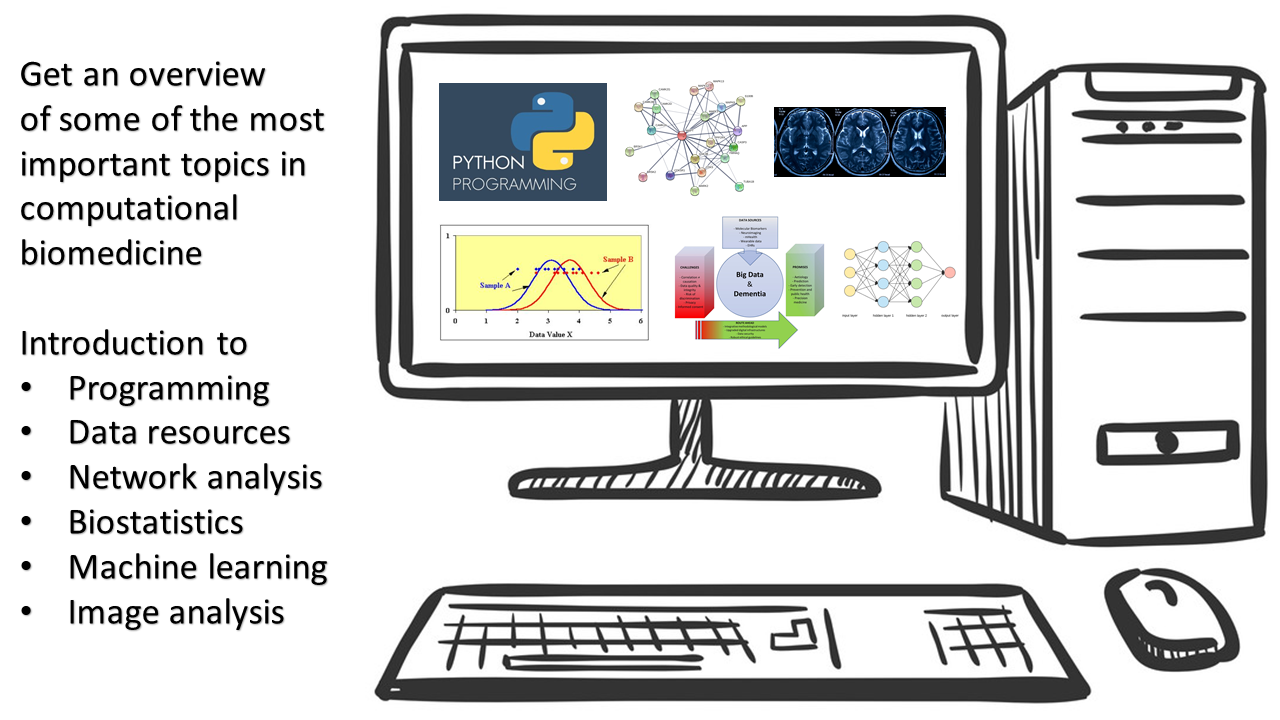
\includegraphics{assets/overview.png}

\hypertarget{learning-objectives}{%
\section{Learning objectives}\label{learning-objectives}}

The aim of the course is to introduce you to important concepts within the field of computational biomedicine as well as to programming. It will provide you with knowledge and ideas that can help you bridge the communication between traditional molecular biologist and computational biologists, and hopefully inspire you to how you can use computational biomedicine in your own research.

This course does not claim to make you an expert within computational science, or train you to do sophisticated programming on your own. These are skills you would need to develop further in follow-up courses or projects. However, we hope that the relevance and practical challenges \& solutions become easier to connect with theory by going over the exercise materials.

\hypertarget{future}{%
\section{Future}\label{future}}

Computational biomedicine is a rapidly growing and evolving field. This is partly due to the changes - or paradigm shift - going on in the fields of cell and molecular biology: a change from a reductionist approach with focus on the biology of a single or a few components to a much more integrative approach where we look at systems biology. This change is highly driven by the development within computer science and large-scale studies in the fields of genomics, proteomics, imaging etc. producing ``big data'' that needs to be integrated in order to obtain relevant and important knowledge within biomedicine. Traditional molecular biology researchers therefore needs to team up with experts within the fields of computational sciences and develop advanced computer algorithms, databases, statistical tools and mathematical models. Such interdisciplinary studies are the way forward for development of e.g.~personalized and predictive medicine and precision diagnostics tools.

\hypertarget{introduction-to-computational-biomedicine-and-machine-learning}{%
\chapter{Introduction to Computational Biomedicine and Machine Learning}\label{introduction-to-computational-biomedicine-and-machine-learning}}

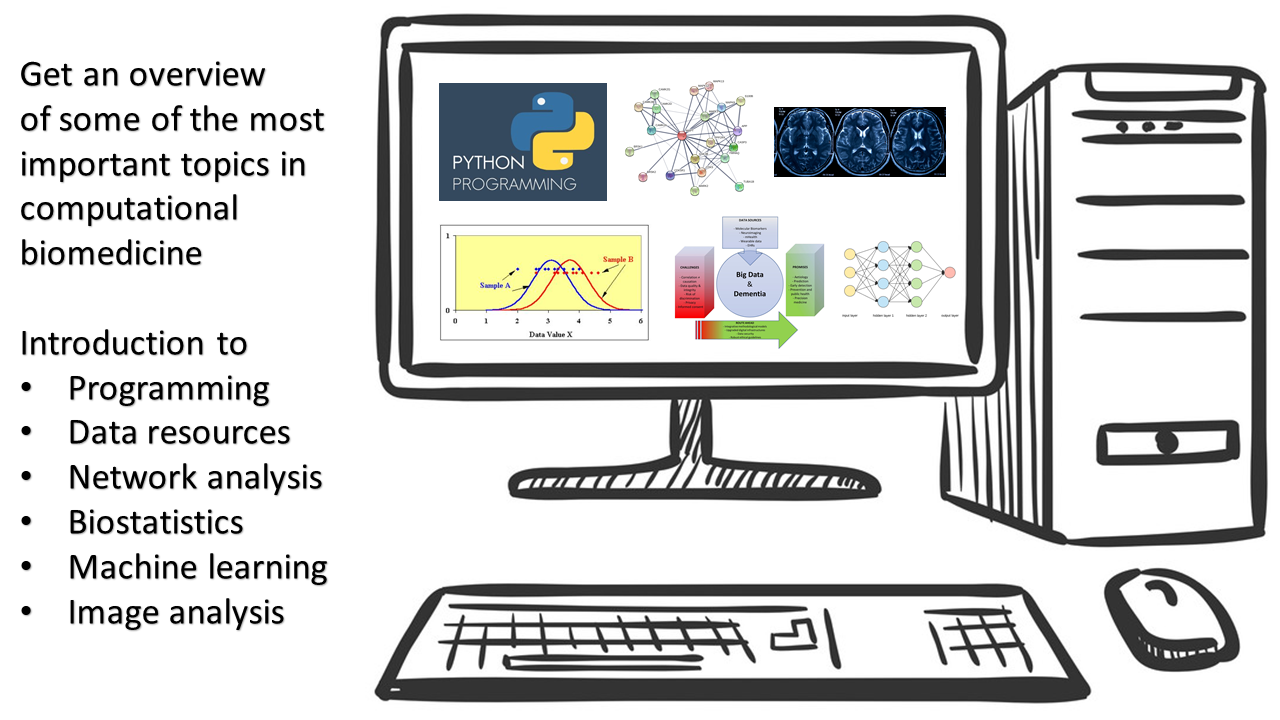
\includegraphics{assets/overview.png}

Short summary

This book accompanies course materials that we share via GitHub. The materials have been put together with the goal to introduce computational biomedicine to students who may enroll to Biomedicine curriculum programs, however we have also used the materials to teach computational students about possibilities of different methods in context of biomedical applications.

The material covers important tools and data resources in this field, and through applications we aim to demonstrate what basic knowledge in network analysis, mathematical models, statistics and machine learning is needed to work with and understand results from high-throughput biomedical experiments (imaging and omics). For each topic there are hands-on data analysis exercises in Jupyter notebook format and this book is meant to cover some basic background related to each exercise.

\hypertarget{what-is-this-course-about}{%
\section{What is this course about?}\label{what-is-this-course-about}}

The quantitative aspect of biology is inherent to biology, although it is often overlooked. This is because Nature is quantitative. The amount of rain that falls on a particular territory, and not only whether it rains or not, dictates the amount/type of vegetation, which eventually dictates the amount/type of animals the territory can feed.

Lord Kelvin expressed his view in 1883, ``When you can measure what you are speaking about, and express it in numbers, you know something about it;
but when you cannot measure it, when you cannot express it in numbers, your knowledge is of a meager and unsatisfactory kind:
it may be the beginning of knowledge, but you have scarcely, in your thoughts, advanced to the stage of science, whatever the matter may be.''

In this introductory course to computational biomedicine we aim to give you an overview of the different steps related to acquisition, processing, visualization and analysis of quantitative data, and its integration in predictive quantitative models.

\hypertarget{systems-biomedicine}{%
\section{Systems biomedicine}\label{systems-biomedicine}}

Systems biology/biomedicine is a conceptual approach, developed to study biological sciences from a quantitative perspective. It is very recent - the first Institute for Systems Biology was created in 2000 in Seattle by Leroy Hood and coworkers, following the first whole genome sequencing results in the late nineties in unicellular organisms. These groundbreaking datasets revealed the enormous complexity of biological systems: eukaryotic genomes are made of millions, if not billions of base pairs, all of which can virtually affect the functioning of the entire organism.

As nicely explained in this video by Dr.~Leroy Hood, researchers at this time needed a way, a state of mind, to conceptually think of entire biological systems in a more global way, as an alternative to the ``older'' reductionist biology/medicine approach that consists in dissecting the components of the system to find molecular targets to cure diseases.

\hypertarget{new-frontiers---explorers-survival-toolkit}{%
\section{New frontiers - explorer's survival toolkit}\label{new-frontiers---explorers-survival-toolkit}}

The first genome of a human individual was sequenced in 2008. This is just a decade ago. So yes, we are, you are explorers on a brand new mountain route. And every explorer needs a survival toolkit. May this course and similar ones be your toolkits!

Specifically, you will develop skills in systems-level thinking, biological network analysis and quantitative biomedicine. You will learn about important programming tools and the basics of biostatistics and machine learning methods, that you will apply to analyze datasets from your own or from data resources, in order to become able to work with and understand results from high-throughput biomedical experiments (imaging and omics).

\hypertarget{systems-level-thinking}{%
\section{Systems-level thinking}\label{systems-level-thinking}}

Let's understand first why it is very, very important to fully appreciate the added value of quantitative and computational tools to biomedicine.

\hypertarget{networks}{%
\chapter{Networks}\label{networks}}

Let's start by an analogy. Let's envision biological systems as train networks.
Video 1

This is what we talk about in the video:
We will be looking at the train network in Finland. Nodes on this network are city train stations, connected by railways. For a cell biologist, these nodes can be genes, proteins, or other biological molecules, connected by molecular interactions, or even cellular states connected by transitions. For a neurologist, they are neuronal cells, connected by synapses. For an ecologist, these nodes are individual species, connected by trophic predator-prey interactions.

\hypertarget{biological-networks}{%
\section{Biological networks}\label{biological-networks}}

Most if not all the current diseases that challenge our therapeutic abilities have cell biological roots, so let's adopt the point of view of a cell biologist. A cellular function is defined by a particular response to a particular stimulus, multiple stimuli, or the absence of stimulus.

It is analogous to a well-defined travel from, for instance Oulu in the north to Lappeenranta in the south. This trip generally involves a train change in Kouvola. For the cellular function to be performed correctly, the Lappeenranta protein node or cellular state has to be activated in due time.

\hypertarget{disease-from-a-network-perspective}{%
\section{Disease from a network-perspective}\label{disease-from-a-network-perspective}}

Diseases occur when the cellular response to the stimulus is not appropriate, in other words when the travel does not end up where or when it should. For instance, activating the Lahti node instead of the Lappeenranta node could mean activating cell proliferation rather than quiescence, leading to cancer.

On cellular level, diseases perturb how messages are propagated (train travelers) propagate throughout the network. Treating a disease is equivalent to being able to counteract network perturbations, in our train analogy to get to Lappeenranta, regardless of the nature of the perturbations. And if possible, not adding more perturbations.

To treat the Lahti node problem, we could just\ldots{} blow up the Lahti station. This way, no train will ever end up in Lahti, or even transit through the station. This is what we do when we use antiproliferative drugs to treat cancer. And clearly, this certainly affects other travelers, other cellular responses to other stimuli, explaining the toxicity of anticancer agents for instance. In addition, it does not guarantee you will get to Lappeenranta. You could even get to a worse node!

So we definitely need a finer approach, and this requires a deeper knowledge of how the train network works.

\hypertarget{identifying-the-functional-modules}{%
\section{Identifying the functional modules}\label{identifying-the-functional-modules}}

\begin{itemize}
\tightlist
\item
  Do you think that a traveler from Oulu to Lappeenranta needs to know all the timetables of all the Finnish trains to circumvent network perturbations and go to destination?
\end{itemize}

Certainly not. But knowing some key railway routes, hub stations, regional subnetworks and the national lines connecting them, and some late trains timetable will certainly help. And this is what systems biomedicine is about: identifying the cellular functional modules, how they are connected and impinge on one another, in order to understand how to pharmacologically manipulate them in a fine, subtle way.

So let's get back to square one, where our cell is an unknown, mysterious land. With genome sequencing efforts, high-throughput computational analysis of the sequences, and further biochemical characterizations, we have identified tens of thousands of cellular network components, like proteins or mRNAs. This data is in large part openly shared to the scientific community through large data repositories.

This is still work in progress, as we are continuously identifying new network nodes, like for instance recently long non-coding RNAs or small ORFs that code for microproteins of a few residues.

\hypertarget{identifying-interactions}{%
\section{Identifying interactions}\label{identifying-interactions}}

\begin{itemize}
\tightlist
\item
  Do you think knowledge of the train stations is sufficient to travel from Oulu to Lappeenranta?
\end{itemize}

Obviously, not. So, in parallel, scientists are using genetics, biophysical, biochemical, cell biological and many other approaches to characterize the interactions between these nodes, the railway routes. A very common approach is to close one station and look which travels are affected, the knock-out approach, or to shut down one railway line and analyze the resulting perturbations, like for instance when a particular protein-protein interaction is disrupted by a controlled point mutation.

And this is where we stand as per 2020. We are progressively revealing a dense network of interactions between cellular objects, and how well-identified disease-causing mutations modify these interactions. We are therefore learning about finer and finer details of the regional and local train networks, and how these networks are structurally altered in disease.

\hypertarget{network-structure-vs-dynamics}{%
\section{Network structure vs dynamics}\label{network-structure-vs-dynamics}}

Yet we lack ways to efficiently circumvent perturbations on our favorite Oulu Lappeenranta route. And indeed, the more node connections we are revealing, the more it becomes clear that this knowledge is both absolutely required, and at the same time insufficient to predict how to pharmacologically control the response of the network to a given stimulus, or ``information''. Indeed, the knowledge of the network structure, for instance relevant proteins and their interactions, does not tell how it is functionally organized to gather, store and process information and signals {[}1{]}. Knowing the network does not tell us where and when the trains are circulating, how the biological information flows through the network.

And because we are talking about information, let's borrow some concepts from information specialists: the journalists. In journalism, a piece of information is considered complete if it encloses the answers to the 6 W's, 6 basic questions:

\begin{itemize}
\tightlist
\item
  Who? What? When? Where? hoW? and Why?
\end{itemize}

The identification of biological network components answers ``who'' does ``what''. In many instances, the information of when, where and in particular how or how much is missing. As explained in details in the next video, this lack of quantitative information can have a very detrimental effect on our understanding of how a given network works. And this precludes our understanding of the ``why'' biological networks are structured the way they are, and are hijacked by well-identified disease-causing network perturbation. The systems biology, or systems biomedicine approach is aiming to understand biological systems at a global, functional level, in order to decipher their design principles.

And this strategy is particularly relevant in medicine. As different individuals from the same species, we have slightly different genomes, and our cellular networks are a tiny bit different. In addition, we have different lifestyles and even the networks of twins are differentially tuned. Thus, the same disease perturbation in different individuals might have different outcomes, and would thus require slightly adjusted treatments. This observation is at the basis of the concept of personalized medicine.

\begin{itemize}
\tightlist
\item
  Does that mean that any treatment, for any disease must be personalized to be efficient?
\end{itemize}

Absolutely not, because despite their differences, our cellular networks share a lot of functional similarities, emphasizing the importance to understand the functional structure of cell biological networks.

Additional reading:
{[}1{]} Nurse, P. (2008) Life, logic and information. Nature 454, 424--426., and the many positive and negative comments on this article.

\hypertarget{quantitative-biomedicine}{%
\chapter{Quantitative biomedicine}\label{quantitative-biomedicine}}

In this video, we continue with the train station analogy. The purpose of this video is to convince you that this quantitative information is a crucial requirement to understand a biomedical problem, in particular at the systems level.

Video 2

Video content:

The complexity of cell biological diseases stems from the fact that many different molecular events can contribute to the physiological perturbations of the disease state. The diverse disease-associated molecular events apply diverse constraints on the cellular network, resulting in quantitative imbalances in cellular states that call for quantitative approaches.

In most biomedical research fields, the 6 basic questions a journalist would ask are only partially answered. The information of when, where and how much of the cellular components are interacting is missing.

Let us come back to our train network analogy. A critical mutation in the Kouvola station like for instance broken eastbound railways could deviate all trains towards Lahti. But alternatively, delays resulting from railway maintenance works much further north could results in afternoon passengers missing the last eastbound correspondence, leaving no other choice that going westbound or staying in Kouvola. In this situation, however, morning passengers would still be able to proceed to Lappeenranta.

\hypertarget{network-components-vs-parameters}{%
\section{Network components vs parameters}\label{network-components-vs-parameters}}

In the presence of a mutation, the network itself is altered. In the presence of a delay in the signal processing, the network is intact. However a change in a quantitative parameter of the network, a delay in train progression, had the same overall effect for the afternoon travelers, but no effect at all for the morning travelers. Hence, in this case, the way the network responds to the perturbation also depends on the timing of the stimulus. From a therapeutic perspective, pharmacologically restoring the broken railway, or adding late trains from Kouvola to Lappeenranta would be two efficient but radically different ways to solve the disease problem in the two situations.

But choosing between these two strategies would require first to know that Kouvola is a hub connection separating networks in south east from south west finland, in other words a connection separating two functional subnetworks. This is not obvious looking at the network structure only, and systems approaches can help identify these kind of hubs.

Another therapeutic strategy that would work in both situations could be to re-route our train way upstream of the Kouvola hub region, through Eastern Finland. Again, the pharmacological implementation of this strategy would require an a priori knowledge of how the northern, eastern and southeastern subnetworks communicate. Moreover, this strategy should be supplemented with additional east-west trains to compensate for the loss of the Oulu-Kouvola connection.

Beyond spatial and temporal parameters, ``how much'' cellular components are present and interact can have a drastic effect on the network response to the stimulus. Assume that in the normal cell, the conductor of the Oulu-Kouvola train changes at the Pieksämäki station, with a new conductor coming from Joensuu and the original one leaving on a train to south west Finland. Assume a sick cell has delays in conveying the second conductor to pieksämäki, then the first one is left with three options: wait, leading to delays at Kouvola, as discussed a minute ago. Keep on its original schedule, leaving our train in Pieksämäki; or carry on, leading to the cancelation of the westbound train. In this scenario, the number of train conductors available in Pieksämäki becomes a limiting factor due to the disease-associated quantitative delays, forcing the cell to make a decision between three choices that will all have detrimental consequences.

Train staff is regularly transported by trains, and these situations are common in train network management. But because the decisional units at the headquarters of the train company have all the information on the current status of the network in hand, and know all the scheduled trains, they can make a wise decision to fix the problem.

In biomedicine, because we don't have all this quantitative information, we can't. In addition, our lack of quantitative knowledge might also confound our analysis of the network structure itself: in the last example, because train conductors are nearly limiting in the normal cell, a perturbation on the Joensuu-Pieksämäki axis shows strong effects on a completely different line. Hence, it might give the impression to the unprepared experimentalist that the Joensuu-Pieksämäki axis is literally on the Oulu Kouvola axis. In fact it is not, but the limitation in the number of train conductors generates an effective strong connection between the Eastern Finland network and the north south axis.

Hence, this naïve analogy between biological and train networks teaches us that it is crucial to learn more about quantitative parameters of the biological networks, in order to devise clever therapeutic strategies that shall target the regulation of multiple distinct functional modules at the systems level. Once we are able to know how many trains take which routes, when, who are the passengers, conductors\ldots{} and so on and so forth, then we will be able to devise efficient therapeutic strategies, certainly involving synchronized regulation of multiple, well-chosen targets and functions. Along the same lines, we recommend reading Yuri Lazebnik's paper ``Can a biologist fix a radio? Or, what I learned while studying apoptosis'', published 20 years ago but still very relevant today {[}2{]}.

Additional reading:
{[}2{]} Lazebnik Y. (2002) Can a biologist fix a radio? Or, what I learned while studying apoptosis. Cancer Cell 2:179-82, and the comments on this article.

\hypertarget{language-barriers}{%
\chapter{Language barriers}\label{language-barriers}}

\hypertarget{descriptive-language---qualitative}{%
\section{Descriptive language - qualitative}\label{descriptive-language---qualitative}}

Biomedical systems are made of cells, cells of molecules, molecules of atoms \ldots etc. The biology language has been developed over centuries to describe macroscopic biological systems, mostly at the qualitative level.

\hypertarget{quantitative-language}{%
\section{Quantitative language}\label{quantitative-language}}

Physics is an example of a quantitative language which can describe molecules, and to describe atoms. In quantum physics the language is that of mathematics.

These language differences stem from the historical distinction between life sciences and physical sciences, and we are now realizing that this distinction does not make a lot of sense.

\hypertarget{programming-languages}{%
\section{Programming languages}\label{programming-languages}}

Furthermore, you are using also another type of language, programming, to write down the analysis steps in a computer-understandable format, because most biological problems cannot be solved by current analytical mathematics.

\hypertarget{interdisciplinary-science}{%
\section{Interdisciplinary science}\label{interdisciplinary-science}}

When you are working on the quantitative analysis of cells - which is what you want to do for doing predictive biomedicine - you are at the crossroads of these languages, all of which have advantages and pitfalls.

There is not, yet, any common language perfectly suited to quantitative cell biology or systems-level medicine that would be understood by experts of all these fields. Therefore, inter-disciplinary communication will require that biologists learn the basic concepts and formal language of quantitative sciences and basic programming skills, and that physicists or mathematicians eager to contribute in transforming future medicine learn some elementary cell and molecular biology concepts. This will enable you to collaborate and communicate with a broad range of specialists, physicists, mathematicians, computer scientists, geneticists, biochemists\ldots{} etc.

Another current challenge in this field is related to what data and tools are available to the community at large (Macklin 2019) . It is an important goal to move beyond single-laboratory efforts to establish a community dedicated to promote compatible data and software usage.

Additional reading:

Computing skills for a biologist (book)

\hypertarget{data-science}{%
\chapter{Data science}\label{data-science}}

Data science focuses on the study of scientific methods for extracting knowledge and insights from data. The techniques and theories come from broad areas of mathematics, statistics, information sciences, and computer science. Machine learning (ML), data mining, and artificial intelligence are an integral part of data science. The three are connected to each other and it may depend on who you ask what that picture looks like (e.g.~some include everything under AI, other draw overlapping circles). To make some distinctions and links, expertise in databases and data management is more often mentioned in context of data mining. Machine learning on the other hand is often seen as an inherent part of data mining and artificial intelligence. However, in AI the ``traditional'' ML is distinguished from deep learning that has its roots in neural networks that spurred a lot of interest already in the 1950s. Deep learning really leaped forward in the 2010s owing to explosion of digital data availability, advances in algorithms and computational power.

Data science is making enormous impact in the biosciences, such as Deepmind's Alphafold to predict protein tertiary structures from sequence, and nothing suggests that its relevance in (bio)medicine will dwindle in the future. Seizing the opportunity early to learn these methods is a great resource for life science researchers.

\hypertarget{learning-from-data}{%
\section{Learning from data}\label{learning-from-data}}

One of the famous definitions of ML is

\emph{A computer program is said to learn from experience E with respect to some class of tasks T and performance measure P, if its performance at tasks in T, as measured by P, improves with experience E.}

In other words, any program that learns about the world from experience. While the term machine learning has blown up in recent years, a more traditional term is \emph{statistical learning}, as most algorithms essentially boil down to clever use of statistics.

How does this differ from conventional programming?

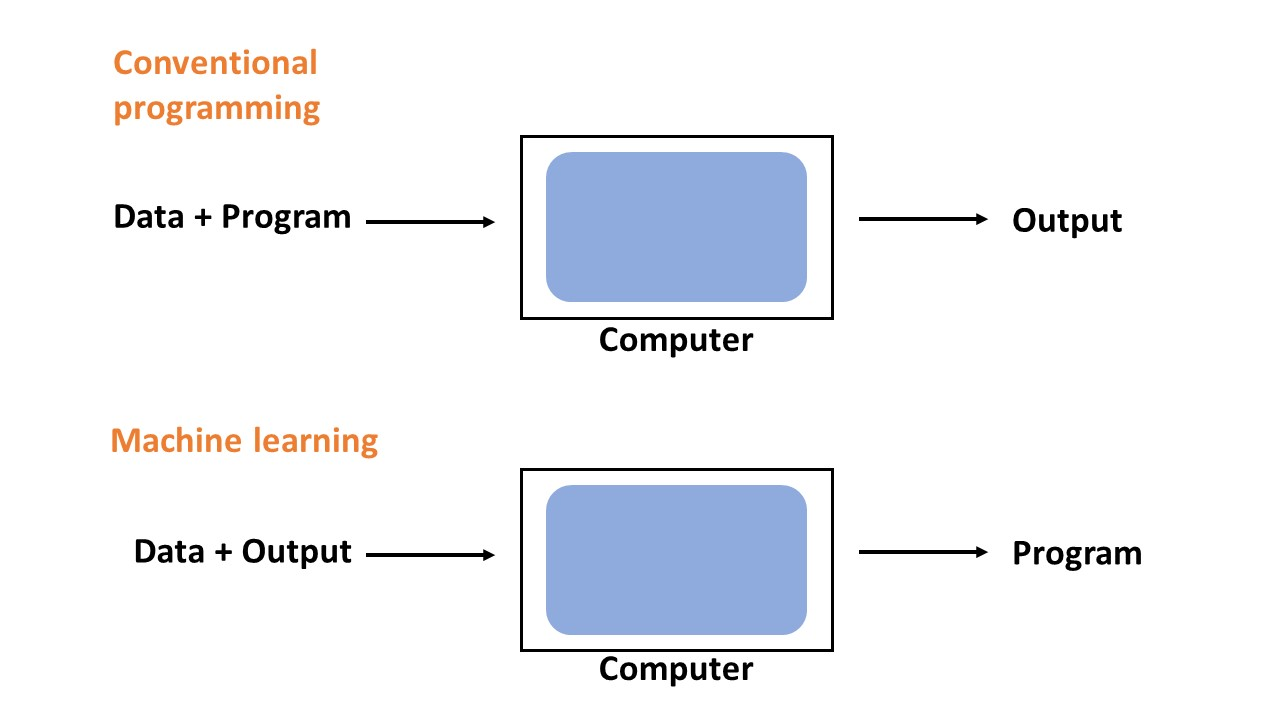
\includegraphics{assets/ml_vs_programming.jpg}

\hypertarget{data-driven-research}{%
\section{Data-driven research}\label{data-driven-research}}

Historically, any type of data analysis was most often performed after data is collected. Today, these approaches are used already earlier, and in this manner they can inform designing new experiments. The transformation that led to this was technological - we can collect whole genome sequences, acquire 3D brain imaging data, or record movies of protein dynamics inside cells. Most importantly, such data are also made available to the scientific community, enabling any researcher to access databases that may host information about every protein inside a cell, or store the original data collected from high-throughput studies. This offers the possibility to use data science methods for discovering interesting patterns or statistical associations in the data, which upon visualization might reveal insight on biology that can then be used to propose hypotheses to be tested in new experiments.

Later, in the statistics perspective section we will re-visit this as we discuss conventional scientific hypothesis testing.

\hypertarget{inspired-by-the-brain}{%
\section{Inspired by the brain}\label{inspired-by-the-brain}}

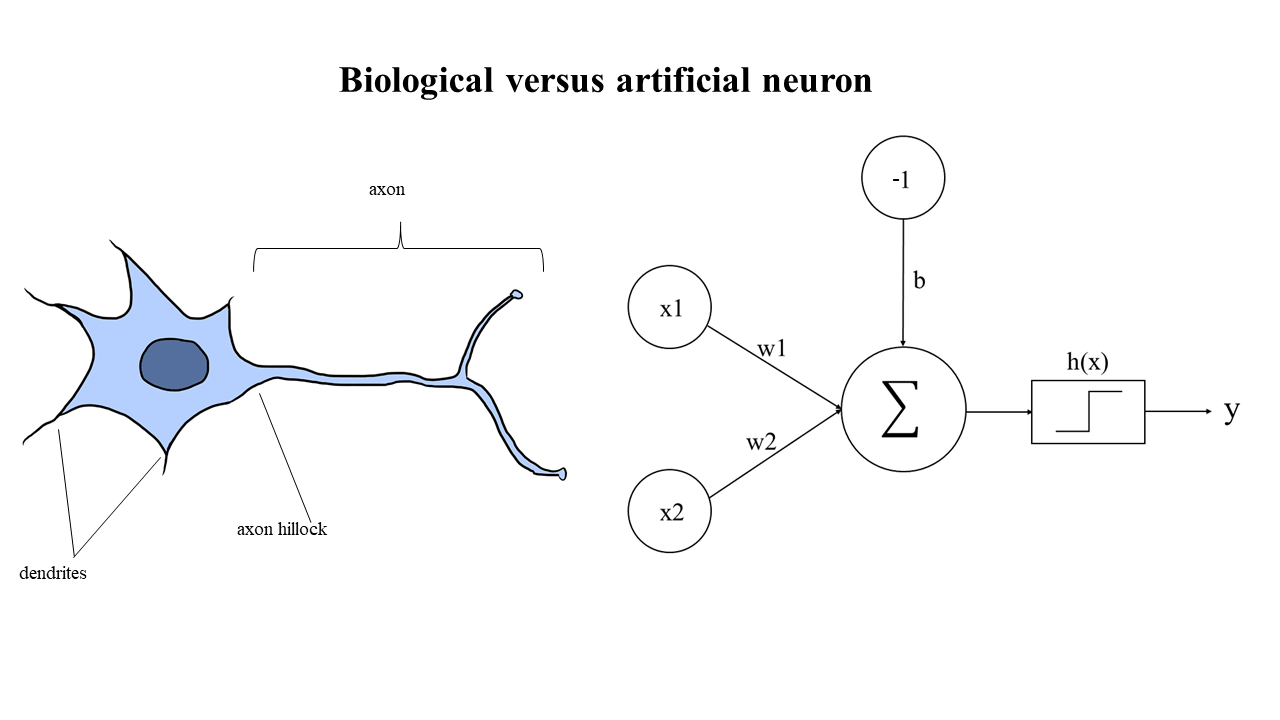
\includegraphics{assets/neuron_artificial_biological.png}

Artificial Neural networks (NNs) make up a subset of algorithms within the broader category of machine learning. Broadly speaking, NNs can be thought of as simple models of biological neural systems, in which layers of neurons propagate information from input to output, facilitated by connections (``synapses'') between the neurons in adjacent layers. We model them simply enough as matrix multiplications. These networks can learn by adjusting the synapse strengths, much like the way animal brains learn through long term potentiation.

They are extremely versatile in that the possible variation in model (the number and type of interconnected layers of neurons, and how many neurons per layer) is virtually endless.Neural networks can for example be taught to perform classification, just as animal brains are extremely powerful to classify the information they receive and make decisions based on it (e.g., is it a mouse or a tiger that is just in front of me?). Provided with enough data, they now consistently outperform traditional ML models.

In this course, we also discuss interdisciplinary paths - the discussion of Andrew Ng and Geoffrey Hinton (both very influential in the field of AI) in this video reveals that Geoffrey got influenced by many different fields in his path towards the innovations in AI that is now famous for.

\hypertarget{data-representation}{%
\section{Data representation}\label{data-representation}}

Next, we introduce a few important concepts. The main point is not for you to memorize everything, but to expose you to concepts that you will encounter later if you take a data science course.

\emph{Feature space} What is data? Depending on who you ask you might get a different answer, but for ML purposes we can usually describe a single data point as a vector of numbers, each number representing the value of some feature. An example of a numerical feature could be continuous like height or a price of a product, or discrete like the number of mutations in a gene. Non-numerical features could include your preference in movies or whether or not you use tobacco. All these features not only can, but actually require to be represented numerically before you can start to do machine learning.

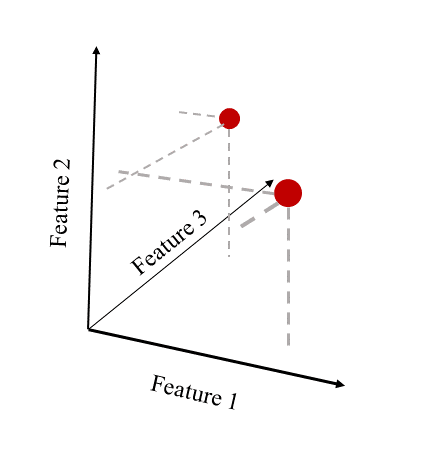
\includegraphics{assets/feature_space.png}

In an abstract manner, we can visualize each feature as spatial dimension, and each data point is simply a point in this space, referred to as feature space. Often we have tens or hundreds of features, and it is easy to lose intuition. Nonetheless, realizing that almost all data can be represented in this very generic manner, we can easily conceptualize any problem within this framework, whether it be health related data, shopping habits or government intelligence and crime statistics.

\emph{Overfitting}
Machine learning can almost always be abstracted to the fitting of a mathematical function to some experimental data. Intuition will have it that the closer we fit to our data points, the more successful we are. This intuition however is only true up to a certain point. After this point, we are essentially ``perfecting'' our model on trying to predict random noise and outliers. The image below clearly explains why a perfect fit usually is a symptom of overfitting: the blue line would severely misjudge the training point (red) between -5 and -4. For this reason, a simpler linear model is preferred: despite getting some of the training points wrong, it generalizes better, i.e.~it would allow to make better predictions about unseen data.

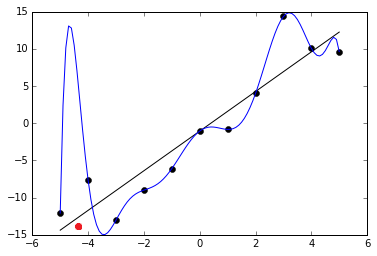
\includegraphics{assets/Overfitted_Data_Ghiles_CCBYSA4_0.png}

Overfitting is the antithesis of proper generalization. As an analogy of overfitting, you can imagine a student who intensively memorizes every fact without genuine understanding, and thereby performs poorly on new problems (but near perfect on already seen ones). This is exactly how you can spot overfitting: you always keep some of the data you have for testing and when training the model this test data is not used. Then you compare the model performance both in training and test sets. If the model is overfitted, the test error is much higher than the training error. Keep in mind though, that underfitting is also a possibility. In this case, you have selected a too simple model.

\emph{Parameters and hyperparameters}
After a model has been selected, ML is all about finding a set of parameters which reduces what is known as the error function (cost function, see below). For instance in linear regression, the parameters are the coefficients of the regression line (what is actually being learned). This optimization of what value to select for each parameter is what the ML algorithm automatically finds. Another set of parameters, hyperparameters have to be predefined prior to training the model, and usually relate to the way the model is trained (for instance, what should the rate of learning be).

\emph{Cost function}
It is always useful, and often necessary to quantify the model error. This is usually some variation of the deviation between prediction and ground truth (e.g.~mean squared error, MSE). While training our data, we are looking for the model parameters which make the error as small as possible. We thus formulate a function, the cost function (also known as loss function), which is a function of the model parameters. The way a model is fitted (or trained) to some data is (explicitly or implicitly) through reducing the cost function. Just like we above conceptualized data features in a hyperdimensional feature space, we can do the same with model parameters. Thus we can imagine a hilly landscape in 3 dimensions, where the x- and y-axis components (e.g.~GPS coordinates) represent the parameter values, and the z-axis component (altitude of each point) represents the error. Different models have clever ways to navigate in this parameter landscape in order to reach a local minimum, like a saddle or a valley. Notice however that there might not be a guarantee that the minimum reached is the global minimum, for instance the sea level.

\emph{Model complexity}
A useful distinction between models can be made by considering their complexity. Note that the word ``complex'' is not synonymous to ``complicated''. Complexity simply refers to something composed of many parts. In this context, complexity is related to the number of parameters the model holds. The more parameters we have, the more complex is our model. Simple linear regression has a low number of parameters, but neural networks (especially deep neural networks) have plenty. When doing machine learning, you should generally test multiple models, always starting with the less complex (although more `boring') alternatives. The reason for this is the general tendency for complex models to overfit as well as requiring more training data. A topic that usually comes up in discussions of complexity is bias-variance tradeoff: complex models have usually a low bias, but a high variance. Simple models have it opposite.

\emph{The curse of dimensionality}
Another common problem relates to the number of features (dimensionality) of the input data. Consider a 2-dimensional input space, where each feature can take the value 0,1 or 2. There are a total of 3\^{}2=9 combinations of inputs. As we increase dimensions from 2 to 3 dimensions, we drastically increase the number of possible combinations of inputs from 9 to 3\^{}3=27. Usually the dimensionality far supersedes 3 dimensions. If we want to get a representative sample of this state space, we need exponentially more and more training samples. Even more, many of the features will be completely irrelevant to our final prediction. This makes training on high-dimensional data challenging, but there are methods to deal with it (incl.~dimensionality reduction).

\emph{Preprocessing}
A model can never be of higher quality than the data it has been trained on. This can be summarized in the mantra ``Garbage in, garbage out'', putting a well-deserved emphasis on ensuring that your data is of decent quality. Moreover, many ML models require the data to come in a certain format, or to be normalized first. In fact, a staggering amount of time of a machine learner's time goes to preparing the data to be modelled. For these reasons we need to review the data. Images should be plotted and inspected, tabular data should be plotted (histograms, line plots etc). It can also be useful to make note of the mean and median values (if the data is numerical), or normalize it (neural networks require normalization). For non-numerical data (such as classifications of healthy or sick), we need some way to translate the categories into numbers, so they can be understood by a computer. For simple problems,we can simply replace the category with a `1' or a `0', while other problems require slightly more elaborate schemes (e.g.~one-hot encoding).

\emph{Feature selection and extraction}
Traditional machine learning requires manual feature selection: you as a scientist need to decide which features you want to gather or use as input to your ML model. There are also statistical techniques to select the ``best'' (most predictive) features from a dataset. Another related concept is feature extraction, in which new features are created by combining the available ones. This is often done through dimensionality reduction. In modern deep learning, feature selection and extraction has become minimal, by letting the algorithm do it automatically. This is known as feature learning.

\emph{Regularization}
The sensitivity of many learners to overfit can be handled using various techniques, colloquially known as regularization. Regularization techniques are used widely in linear regression to make it robust against outliers and noise, known as L1 and L2 regularization. Neural networks may also be regularized using dropout (random removal of neurons).

\hypertarget{physical-vs-statistical-model}{%
\section{Physical vs statistical model}\label{physical-vs-statistical-model}}

You may be wondering how the data science approach connects with systems-level thinking? This is actually an open question. However, there are interesting possibilities for synergy. As food-for-thought, here is a Nature article discussing this in context of trying to understand how the Earth behaves, as a system. This article brings up the distinction where physical modelling and machine learning have been seen as two different fields with very different scientific paradigms (theory-driven versus data-driven). In the physical approaches, physical laws are combined to draft causal models where a certain feature (for instance, the gravity force from the moon), has a certain effect (ocean tides). Therefore, physical approaches are in principle directly interpretable and offer the potential of extrapolation beyond the observed conditions. But the quality of the predictions is generally tied to the limited number of ingredients that have been accounted for in the model. In contrast, data-driven approaches are highly flexible in adapting to data that has been collected and are amenable to finding unexpected patterns (surprises). But interpretation, and in particular causality, is often harder to infer. A classic example drawn from ``The Visual Display of Quantitative Information'' textbook by Edward Tufte illustrates the difficulty of interpreting statistical correlations:

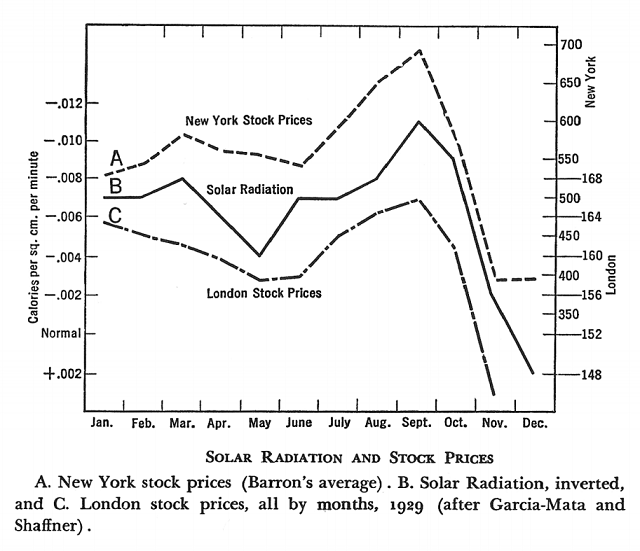
\includegraphics{assets/StockvsRadiation.png}

Can we safely believe that the solar activity causes fluctuations in the stock market? For these reasons, physical (or biological) and statistical models can also be synergistic!

Additional reading:

Marx 2009. Machine learning, practically speaking

An Introduction to Statistical Learning (book)

\hypertarget{statistics-perspective}{%
\chapter{Statistics perspective}\label{statistics-perspective}}

Compared to data science, using statistics has long history in research. The goals could be summarized as:

Describe: summarize data in a simplified way that we can understand

Decide: make decisions based on data, in the face of uncertainty

Predict: make predictions about new situations based on our knowledge of previous situations

Let's consider an example where we have data across 100 000 study participants (which we call the sample) regarding their vitamin D levels. We also have the health records available and would be interested to study association between the vitamin levels and disease prevalence, for example.

Compared to machine learning, statistics tries to make the data better understandable for a human. Given our study of 100,000 people, one way to describe this data in a simple way is to divide the data into groups, after ordering them in terms of their intake of vitamin D; the first quantile contains the 20\% of people with the lowest intake, and the 5th quantile contains the 20\% with the highest intake. Now, instead of 100,000 data points, we could plot vitamin D intake level (categories) against cancer-related deaths. In fact, one way to think about statistics is aggregation, i.e.~we throw away details of the study participants and make conclusions based on data summaries that consists of a small set of ``data metrics'', or statistics (e.g mean and standard deviation, or reporting quantiles).

If we indeed observed a trend between vitamin levels and cancer based on our summary, we might want to proceed to evaluate this relationship further. There is a lot of uncertainty in the data, in any real-world dataset; for example, it would be normal to have some people with high vitamin intake who died of cancer, and, similarly, some people with very low intake who never had cancer. Given the observed variability, we want to \emph{decide} whether the trend we see in the data is large enough that we wouldn't expect it to occur randomly \emph{if there was not truly a relationship} (null hypothesis) between vitamin intake and cancer incidence. Statistics provide the tools to make these kinds of decisions.

\hypertarget{statistical-models-and-scientific-hypotheses}{%
\section{Statistical models and scientific hypotheses}\label{statistical-models-and-scientific-hypotheses}}

Below you find a set of steps that we generally go through when we want to use a statistical model to test a scientific hypothesis (\emph{decide} to accept or reject it):

\begin{enumerate}
\def\labelenumi{\arabic{enumi}.}
\tightlist
\item
  Specify your question of interest
\item
  Identify or collect the appropriate data
\item
  Prepare the data for analysis
\item
  Determine the appropriate model
\item
  Fit the model to the data
\item
  Criticize the model to make sure it fits properly
\item
  Test hypothesis and quantify effect size
\end{enumerate}

\emph{Choice of model} Centuries of statistics research have provides guidelines that can help decide what type of models are suitable for which type of data and questions. For example, a normal distribution fit could be a good model to capture key properties (such as expected value) for continuous valued measurements but not appropriate for discrete data such as counts.

One such example is sequencing data! Before, in the 1990s when microarray technology was used to compare gene expression levels in biological samples, researchers could utilize the powerful statistics tools available for continuous (log)-normal data, including linear models. The whole workflow had to be ``re-invented'', i.e.~built around a different toolset suitable for discrete data, when sequencing-based count data from RNA-seq became common.

\emph{The good and bad p-value} The idea of following steps 1-7 is very logical. However, it turns out that it is more difficult to publish results when the study concludes that the hypothesis proposed initially should be rejected (negative results). Similarly, expensive experiments have led to design of ``minimalistic'' studies where we attempt to make conclusions based on smallest possible sample sizes. This has led to many problems, referred to as p-hacking. So a word of caution is at place here about the pitfalls you should avoid:

p-hacking is if you:

-Analyze data after every subject, and stop collecting data once p\textless0.05

-Analyze many different variables, but only report those with p\textless0.05

-Collect many different experimental conditions, but only report those with p\textless0.05

-Exclude participants to get p\textless0.05

-Transform the data to get p\textless0.05

Any of the above, corrupts the whole scientific process, as no real conclusions can be drawn.

\hypertarget{probability}{%
\section{Probability}\label{probability}}

Probability is the branch of mathematics that deals with chance and uncertainty. Instead of going after some arbitrary p-value threshold, it is much more useful to accept that there is uncertainty in our conclusions, for example by including confidence intervals, and using concepts from probability theory.

You might associate probabilities with the calculations you learned in school for experiments such as rolling a dice, where a certain number of possible outcomes are possible. Then you apply the calculation on a certain observed sequence of events (sample). Alternatively, you could be observing passing cars at the intersection and recording those that are electric cars.

Many biomedical experiments involve sampling and can be related to the ``classical probability'' experiments. For example, a blood sample where we count certain cell types is similar to the ``electric car counting'' situation, and mathematically a model (probability distribution) has been proposed that allows you to calculate the probability of observing a certain number of events (e.g.~T-lymphocytes) per fixed time/volume (1 ml of blood sample), if we know how many to expect on average. A Poisson model can be used to calculate the probability of a given number of events occurring in a fixed interval of time or space, i.e.~it would be appropriate for the situation above. The choice of the ``model'' is based on the type of experiment that was performed.

From this basic foundation, an interesting path of probability theory emerges - this idea was so revolutionary that it led to two different statistics ``schools'' - the frequentists and Bayesians. To get an idea what the difference is, it is first important to understand conditional probabilities, from which the Bayes' rule is derived. We will not go into details here but instead ask - Why is this interesting? In simple words, the Bayes rule gives us a mathematical way to update our beliefs on the basis of data .

Frequentists interprets probabilities ``in long-run'' i.e.~in situations where we can sample many times (or indefinately), e.g.~coin flip. This is less useful if the event can only happen once. For Bayesians probability is as a degree of belief in a particular proposition. This would be better-suited e.g.~to answer at the start of the Covid-19 pandemic in 2019 ``How likely will we have a vaccine developed during 2020?''. The frequencies to calculate the frequentist probability were not available. Based on our prior beliefs (e.g.~how long it took historically to develop vaccines) and knowledge (e.g.~how many labs worked on it then, how many succeeded, and how many would be trying to develop the drug now), we could propose a Bayesian probability calculation for this situation.

\emph{Predicting} is important concept in statistics which is also encountered in machine learning. In both, the idea is to fit a model to the data collected. It is good to keep in mind that when we want to generalize from the data we already have to some other situation, we assume that the particular sample that we have available is representative of a larger population.

Models (and predictions made based on them) can also be updated when new data is collected (Bayes' rule). Many of the sophisticated predictive machine learning models have their roots in probability theory.

Additional reading:

Statistics versus Machine learning

\hypertarget{sign-up-for-inter-disciplinary-training}{%
\chapter{Sign-up for inter-disciplinary training!}\label{sign-up-for-inter-disciplinary-training}}

In conclusion, \emph{because} modern biomedical challenges involves biological systems that are very complex, multi-scale and multi-parametric, the use of traditional intuition-based scientific methodologies need to be complemented with additional tools. In this brief introduction, we have mentioned systems-level thinking, network analysis, data science tools, biostatistics and machine learning methods, and computer programming as part of this survival toolkit.
These topics are covered in several courses provided in your University, and this knowledge in \emph{quantitative science} in the broad sense can be useful well beyond biomedicine (e.g., road traffic regulation, Earth dynamics \& climate change\ldots). Signing-up to such courses will help you develop inter-disciplinary skills early enough in your career, to provide you with high-flexibility to adjust to various scientific environments and anticipate evolutions in the job market.

\hypertarget{intro}{%
\chapter{How to contribute to the book}\label{intro}}

\hypertarget{r-markdown-instructions-from-bookdown-example}{%
\section{R markdown instructions from bookdown example:}\label{r-markdown-instructions-from-bookdown-example}}

You can label chapter and section titles using \texttt{\{\#label\}} after them, e.g., we can reference Chapter \ref{intro}. If you do not manually label them, there will be automatic labels anyway, e.g., Chapter \ref{methods}.

Figures and tables with captions will be placed in \texttt{figure} and \texttt{table} environments, respectively.

\begin{Shaded}
\begin{Highlighting}[]
\KeywordTok{par}\NormalTok{(}\DataTypeTok{mar =} \KeywordTok{c}\NormalTok{(}\DecValTok{4}\NormalTok{, }\DecValTok{4}\NormalTok{, }\FloatTok{.1}\NormalTok{, }\FloatTok{.1}\NormalTok{))}
\KeywordTok{plot}\NormalTok{(pressure, }\DataTypeTok{type =} \StringTok{'b'}\NormalTok{, }\DataTypeTok{pch =} \DecValTok{19}\NormalTok{)}
\end{Highlighting}
\end{Shaded}

\begin{figure}

{\centering 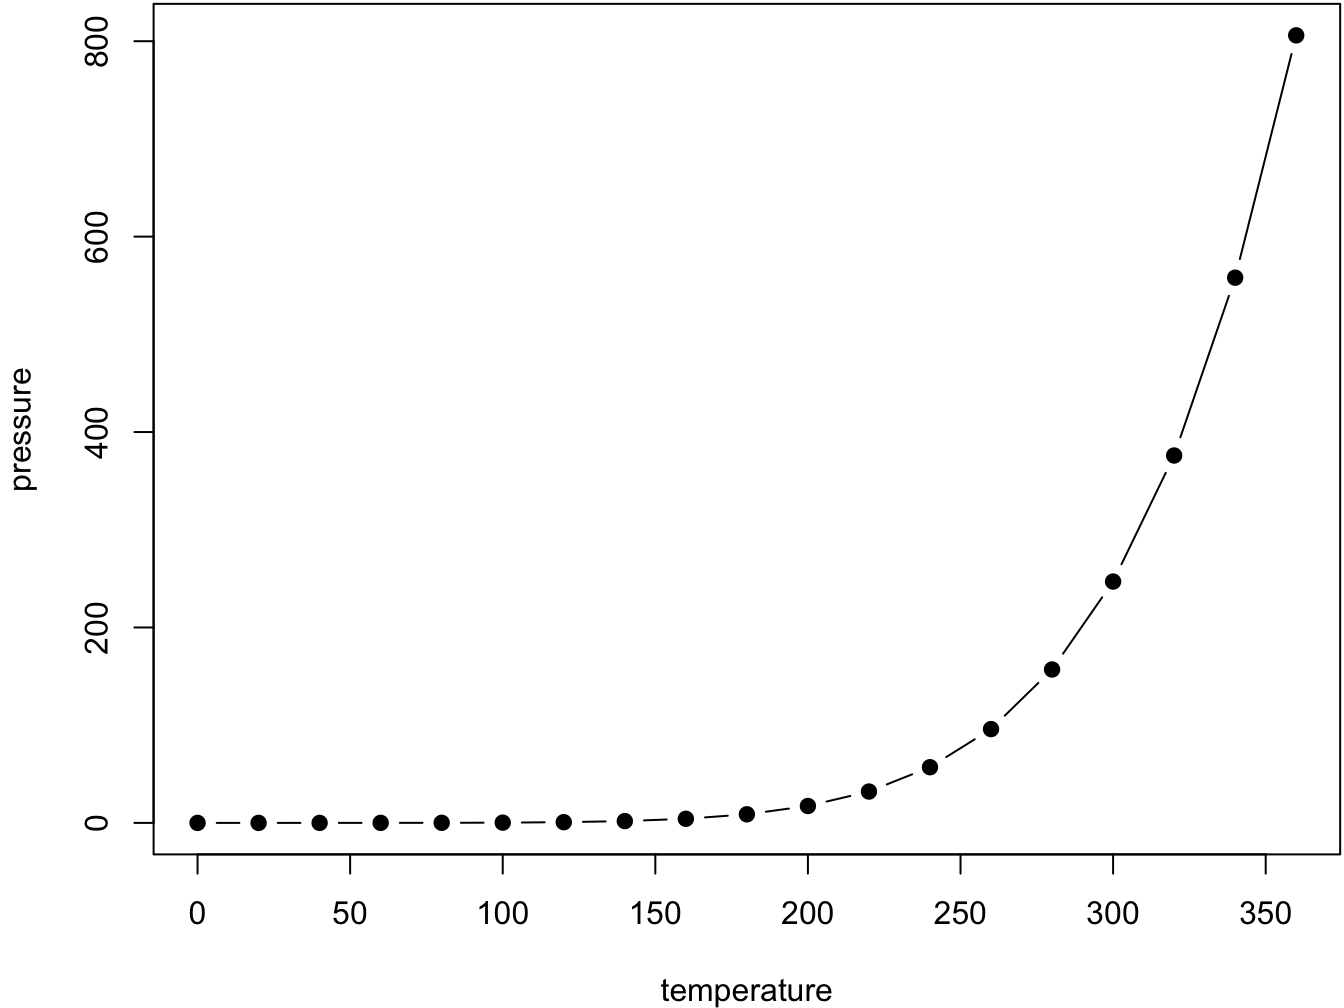
\includegraphics[width=0.8\linewidth]{testBook_files/figure-latex/nice-fig-1} 

}

\caption{Here is a nice figure!}\label{fig:nice-fig}
\end{figure}

Reference a figure by its code chunk label with the \texttt{fig:} prefix, e.g., see Figure \ref{fig:nice-fig}. Similarly, you can reference tables generated from \texttt{knitr::kable()}, e.g., see Table \ref{tab:nice-tab}.

\begin{Shaded}
\begin{Highlighting}[]
\NormalTok{knitr}\OperatorTok{::}\KeywordTok{kable}\NormalTok{(}
  \KeywordTok{head}\NormalTok{(iris, }\DecValTok{20}\NormalTok{), }\DataTypeTok{caption =} \StringTok{'Here is a nice table!'}\NormalTok{,}
  \DataTypeTok{booktabs =} \OtherTok{TRUE}
\NormalTok{)}
\end{Highlighting}
\end{Shaded}

\begin{table}

\caption{\label{tab:nice-tab}Here is a nice table!}
\centering
\begin{tabular}[t]{rrrrl}
\toprule
Sepal.Length & Sepal.Width & Petal.Length & Petal.Width & Species\\
\midrule
5.1 & 3.5 & 1.4 & 0.2 & setosa\\
4.9 & 3.0 & 1.4 & 0.2 & setosa\\
4.7 & 3.2 & 1.3 & 0.2 & setosa\\
4.6 & 3.1 & 1.5 & 0.2 & setosa\\
5.0 & 3.6 & 1.4 & 0.2 & setosa\\
\addlinespace
5.4 & 3.9 & 1.7 & 0.4 & setosa\\
4.6 & 3.4 & 1.4 & 0.3 & setosa\\
5.0 & 3.4 & 1.5 & 0.2 & setosa\\
4.4 & 2.9 & 1.4 & 0.2 & setosa\\
4.9 & 3.1 & 1.5 & 0.1 & setosa\\
\addlinespace
5.4 & 3.7 & 1.5 & 0.2 & setosa\\
4.8 & 3.4 & 1.6 & 0.2 & setosa\\
4.8 & 3.0 & 1.4 & 0.1 & setosa\\
4.3 & 3.0 & 1.1 & 0.1 & setosa\\
5.8 & 4.0 & 1.2 & 0.2 & setosa\\
\addlinespace
5.7 & 4.4 & 1.5 & 0.4 & setosa\\
5.4 & 3.9 & 1.3 & 0.4 & setosa\\
5.1 & 3.5 & 1.4 & 0.3 & setosa\\
5.7 & 3.8 & 1.7 & 0.3 & setosa\\
5.1 & 3.8 & 1.5 & 0.3 & setosa\\
\bottomrule
\end{tabular}
\end{table}

You can write citations, too. For example, we are using the \textbf{bookdown} package \citep{R-bookdown} in this sample book, which was built on top of R Markdown and \textbf{knitr} \citep{xie2015}.

  \bibliography{book.bib,packages.bib}

\end{document}
